\chapter{Young Entrepreneur Interviews SHAQ}

The source interview is from School of Hard Knocks and is curated in this volume by LazyingArt LLC. It is not a chalkboard lecture, and no validated mathematical screenshots survive for this chapter, but the conversation has a clear quantitative spine. We follow the interview in its spoken order: a teaser about 155 franchise locations, a reset in Atlanta, a full interview about imitation, wealth preservation, business ownership, negotiation, delegation, missed opportunity, belief, and advice for beginners. The notes below treat the numbers as evidence from the transcript and use only modest reconstruction where it helps expose the operating mechanism.

\section{Fame Is Not the Mechanism}

The opening is deliberately compressed. The interviewer asks, ``Who am I here with today?'' and the answer is direct: Dr. Shaquille O'Neal. Then the categories arrive quickly. Asked which industry he pursued, Shaq first says, ``A lot of them.'' In the fuller interview he names DJing, law enforcement, food and beverages, and pizza.

That opening might look like a celebrity inventory, but the chapter should not read it that way. The real question is mechanical: how does one person's career income become contact with many businesses? What has to be true for a single owner, with one body and one calendar, to be connected to a large operating surface?

The teaser gives the number that forces the question. The interviewer says Shaq owned 155 Five Guys locations at one point, and Shaq says he sold them. We record the number as an interview claim:

\begin{equation}
N_{\mathrm{Five\ Guys}} = 155.
\end{equation}

A number like \(155\) already defeats direct personal supervision. It is not just ``work harder.'' If the owner must personally appear at each location, the system is impossible before it begins. So the interview turns almost immediately from fame to operating capacity.

\section{Delegation And The 155-Place Constraint}

The interviewer asks for the secret to scaling in the franchise model, or in business generally. Shaq's answer is one word: delegation. Then he gives the reason in physical language: he cannot be in 155 places at once, but he knows somebody who can.

Let \(N\) be the number of locations and let \(C_{\mathrm{one}}\) be the number of locations one person can directly supervise in a meaningful way. The obstruction is simply

\begin{equation}
N_{\mathrm{locations}} > C_{\mathrm{one}}.
\end{equation}

For \(N=155\), the owner cannot be the whole operating system. The only way to make the inequality workable is to add trusted operators. If operator \(i\) can responsibly cover capacity \(c_i\), and there are \(m\) such operators, the reconstructed condition is

\begin{equation}
N_{\mathrm{covered}} \leq \sum_{i=1}^{m} c_i.
\end{equation}

This is not a board equation from the video. It is the clean mathematical skeleton of the spoken claim. Scale is not being everywhere. Scale is building a system in which capable people can be somewhere for you.

\begin{figure}
\centering
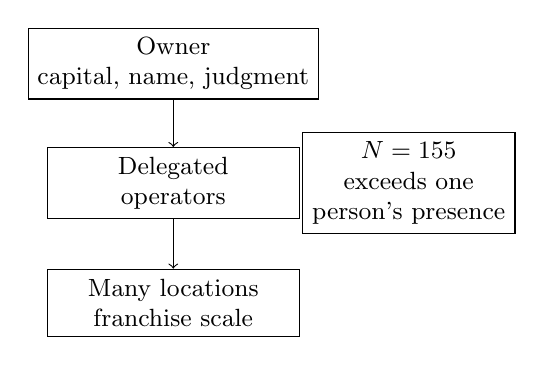
\begin{tikzpicture}[scale=0.92, every node/.style={font=\small}]
\node[draw, align=center, minimum width=3.2cm, minimum height=0.85cm] (owner) at (0,0) {Owner\\capital, name, judgment};
\node[draw, align=center, minimum width=3.2cm, minimum height=0.85cm] (ops) at (0,-1.65) {Delegated\\operators};
\node[draw, align=center, minimum width=3.2cm, minimum height=0.85cm] (sites) at (0,-3.3) {Many locations\\franchise scale};
\draw[->] (owner) -- (ops);
\draw[->] (ops) -- (sites);
\node[draw, align=center, minimum width=2.7cm, minimum height=1.0cm] at (3.25,-1.65) {\(N=155\)\\exceeds one\\person's presence};
\end{tikzpicture}
\caption{A transcript-derived reconstruction of the delegation mechanism. The owner remains important, but operating capacity must pass through other people.}
\end{figure}

\subsection{Question \& Answer}

\paragraph{Question.}
How can one owner scale beyond personal attention?

\paragraph{Answer.}
By separating ownership from direct presence. The obstruction in the interview is physical: one person cannot be in 155 places at once. The resolution is organizational: choose operators who can carry local execution. The owner still supplies capital, reputation, strategic direction, and judgment about people, but the work is distributed.

This is why the interview later returns to championships. A championship team is not a decorative metaphor. It is the pattern Shaq uses to explain business scale: great outcomes require capable people in the right roles.

\section{Model Theft And Skill Transfer}

After the opening teaser, the host resets the story. They have landed in Atlanta, and Shaq is framed as both one of the great basketball players and a business mogul, with the host claiming a net worth above 500 million dollars. Then the interview begins again in full: name, industries, prior career, and success.

The serious turn comes when the interviewer asks about the biggest driving factor in Shaq's career. Shaq says, ``I was a thief,'' and then defines the term. If someone is doing better than you, and you aspire to be like them, steal what they are doing. He names Michael Jordan, Magic Johnson, Kareem Abdul-Jabbar, and Muhammad Ali, then says he put those influences inside his brain and created Shaquille O'Neal.

We should not over-formalize the line, but it has a useful structure. Let \(M_j\) be a model, and let \(s_j\) be a skill, habit, posture, or operating discipline extracted from that model. A cautious update rule is

\begin{equation}
\mathrm{Self}_{t+1}
=
\mathrm{Self}_{t}
+
\sum_{j=1}^{k} w_j s_j
+
r.
\end{equation}

Here \(w_j\) is the weight given to model \(j\), and \(r\) is the irreducible personal remainder: taste, temperament, timing, and what Shaq later calls adding your own ``razzmatazz.'' The transcript's lesson is sharper than the notation: observe, steal, combine, become.

\section{Keeping Money After Making It}

The interviewer then changes the problem. He says athletes can receive large sums and still lose them, citing a claim that one in three NFL players go broke within three to five years. We keep that as a spoken claim by the interviewer, not as a verified statistic:

\begin{equation}
\mathrm{claimed\ broke\ rate}
=
\frac{1}{3}
\quad
\mathrm{within}
\quad
3\text{--}5\ \mathrm{years}.
\end{equation}

The question is how to preserve wealth when a lot of money arrives at once. Shaq's answer is short: for those who are not financially literate, learn the word annuity. He does not give a detailed finance lesson. The note should not pretend that he did. But we can mark what the word does in the conversation. It turns a lump into a governed stream:

\begin{equation}
W_0 \longmapsto (P_1,P_2,\ldots,P_T).
\end{equation}

The symbol \(W_0\) denotes initial wealth, and \(P_t\) denotes scheduled payments over time. This is a standard reconstruction of the concept, not a transcript quotation. The point is that a lump sum is not automatically durable wealth. It becomes durable only when governed by structure, literacy, and restraint.

\subsection{Question \& Answer}

\paragraph{Question.}
Why is making money easier than keeping money?

\paragraph{Answer.}
Because making money can happen as a single event, while keeping money is a repeated discipline. Shaq gives two pieces of evidence. First, he points to annuity as a preservation concept. Later, he recalls the first time he received a million dollars: he says he spent it in about 30 minutes on cars, jewelry or similar items, and suits, while not yet knowing what FICO was. The contrast is the chapter's preservation lesson: receiving wealth and having a system for wealth are different things.

\section{Starting, Franchising, And Operating Humility}

The interview is interrupted by a mentorship promotion. It names the School of Mentorship and gives examples such as Steven Klubeck, James Keyes, and Cody Sperber. We should treat that as show context rather than Shaq's testimony. Its useful function is to reinforce one theme already present in the interview: proximity to experienced operators is treated as a form of economic leverage.

When the interview resumes, the host asks whether someone today should start a business or franchise a business. Shaq answers: both. Start when you are inspired by something, want to do it, think it will work, and believe it will work. Franchise, or imitate a proven format, when something is already working and the local opportunity makes sense.

The host then gives another numerical claim: eight out of ten companies go out of business in five years. Again, this is transcript evidence, not external verification:

\begin{equation}
\mathrm{claimed\ failure\ rate}
=
\frac{8}{10},
\qquad
\mathrm{implied\ survival\ rate}
=
\frac{2}{10}.
\end{equation}

Asked for the most common mistake business owners make, Shaq says they think they know it all. His correction is to hire people who are smarter than oneself. This returns us to delegation, but with a sharper condition. Adding people is not enough; the added people must increase the intelligence and operating capacity of the system.

\section{Negotiation Arithmetic And Money Discipline}

The interview then becomes numerically precise. Asked for negotiation advice, Shaq gives two rules: do not talk first, and start high. His example is a compact worked calculation.

Let the other side's budget be

\begin{equation}
B = \$200\mathrm{M}.
\end{equation}

If the opening ask is too low,

\begin{equation}
a_0 = \$50\mathrm{M},
\end{equation}

then the possible value left outside the opening ask is

\begin{align}
L
&= B-a_0 \\
&= \$200\mathrm{M}-\$50\mathrm{M} \\
&= \$150\mathrm{M}.
\end{align}

This is the cleanest arithmetic in the interview. The point is not merely that a high ask sounds confident. The point is that a low anchor can destroy the negotiator's own upside before the negotiation has started.

The transcript also gives a bargaining path:

\begin{equation}
\$200\mathrm{M}
\rightarrow
\$110\mathrm{M}
\rightarrow
\$140\mathrm{M}
\rightarrow
\$125\mathrm{M}.
\end{equation}

It is conversational, not a formal bargaining theorem, but the mechanism is visible: the opening number shapes the field on which the later numbers move.

The same part of the interview gives a savings rule Shaq says he received from a mentor: save 75 and have fun with 25. If \(I\) denotes income, \(S\) savings, and \(F\) fun or discretionary spending, the rule is

\begin{equation}
S = 0.75I,
\qquad
F = 0.25I,
\qquad
S+F=I.
\end{equation}

Again, this is not a universal theorem. It is a discipline. It makes preservation visible by assigning a fraction before emotion and momentum spend the whole sum.

\section{Risk, Teams, And Investment Criteria}

The interview returns to the 155 Five Guys example. Shaq repeats the delegation logic, and then explains that he learned it by winning championships. The basketball lesson becomes a business lesson: having great teammates matters. In our notation, adding operators only works if the \(c_i\) are real capacities, not empty titles.

Then the host asks about the biggest risk Shaq ever took in business. Shaq answers by naming an opportunity he did not take. He says Howard Schultz wanted to open Starbucks in the hood, and Shaq heard the phrase one way. He says he did not yet understand re-gentrification and re-beautification of certain areas, did not pull the trigger, and that Magic Johnson later opened many Starbucks.

The lesson is not that every opportunity should be taken. It is that the words used to describe an opportunity can hide the economic mechanism. Shaq heard one meaning of the neighborhood. The opportunity apparently depended on another meaning: changing places, changing demand, and early positioning.

The later investment rule is simpler. Shaq says successful people are nice, humble, surrounded by great people, and keep things simple. He invokes the idea, attributed in the interview to Jeff Bezos, of investing in things that change people's lives. He also says that when he invests in a person, he wants to believe in what they believe in. So the criterion is not only industry or asset class. It is a fit between usefulness, belief, and the person carrying the work.

\section{Luck, Belief, And The Beginner Blueprint}

Near the end, the interviewer asks how Shaq found the self-belief to make hundreds of millions of dollars. Shaq complicates the question. He says he had an athletic advantage: he was given a lot of money to play sports, then took that money, leveraged it, and did certain things. He says he can kind of answer the question, but not completely, because for him it was luck.

That admission matters. It keeps the chapter source-conscious. The interview contains mechanisms: delegation, imitation, annuity, savings discipline, high anchoring, smarter hires, and investment through belief. But it also contains path dependence. Shaq's starting position included unusual athletic income. The business story begins after that advantage, when he had to learn what to do with money, people, and opportunity.

The final advice returns to the first mechanism of imitation. If you have a plan, write it down and figure it out. If somebody else is already doing what you want to do, watch them, steal what they are doing, and add your own style. Expect ups and downs, and keep believing long enough for the process to work.

The chapter therefore closes where it began. Wealth is not treated as a mysterious glow around fame. It is a sequence of mechanisms: copy useful models, preserve the lump, delegate execution, negotiate from strength, learn from missed opportunities, and keep enough humility to find people who know what you do not.

\section{Summary}

The interview gives a compact theory of commercial judgment. First, there is the 155-place constraint: when \(N\) exceeds one person's direct capacity, delegation becomes necessary. Second, there is the preservation problem: a lump sum becomes durable only through literacy, structure, and discipline. Third, there is the people problem: models, operators, mentors, teammates, and founders all matter because wealth scales through judgment distributed across relationships.

The mathematics in this chapter is reconstructed from the transcript rather than read from board images. That is the right level of formality for this source. The evidence remains the spoken sequence: fame creates attention, but the repeated mechanisms are delegation, preservation, negotiation, belief, and the discipline to keep learning.